\documentclass[12pt]{article}
\usepackage[english]{babel}
\usepackage{natbib}
\usepackage{url}
\usepackage[utf8x]{inputenc}
\usepackage{amsmath}
\usepackage{graphicx}
\graphicspath{{images/}}
\usepackage{parskip}
\usepackage{fancyhdr}
\usepackage{vmargin}
\setmarginsrb{3 cm}{2.5 cm}{3 cm}{2.5 cm}{1 cm}{1.5 cm}{1 cm}{1.5 cm}


							


\makeatletter
\let\thetitle\@title

\let\thedate\@date
\makeatother

\pagestyle{fancy}
\fancyhf{}
\rhead{\theauthor}
\lhead{\thetitle}
\cfoot{\thepage}

\begin{document}

%%%%%%%%%%%%%%%%%%%%%%%%%%%%%%%%%%%%%%%%%%%%%%%%%%%%%%%%%%%%%%%%%%%%%%%%%%%%%%%%%%%%%%%%%

\begin{titlepage}
	\centering
    \vspace*{0.5 cm}
    
\includegraphics[scale = 0.35]{City-Logo.jpg}\\[1.0 cm]	% University Logo
    \textsc{\LARGE CITY UNIVERSITY}\\[2.0 cm]
    \textsc{\lARGE COMPUTER SCIENCE AND ENGINEERING}\\[0.2 cm]
    \textsc{\lARGE MICROPROCESSOR AND ASSEMBLY LANGUAGE LABORATORY}\\[0.2 cm]
	\textsc{\Large CSE 322}\\[0.5 cm]				% Course Code
	\textsc{\large RADIO TRANSMITTED WIRELESS GESTURE CONTROLLED  CAR USING MPU6050 GYRO ACCELEROMETER SENSOR AND ATMEGA328 MICROCONTROLLER }\\[0.2 cm]
	\rule{\linewidth}{0.2 mm} \\[0.4 cm]
	{ \huge \bfseries \thetitle}\\
	
	
	\begin{minipage}{0.4\textwidth}
		
			\begin{flushright} 
			\emph{STUDENT ID :} \\
			141352032\linebreak
			153402341\linebreak
			153402342\linebreak
			141352032\linebreak
			153402301\linebreak
			153402311\linebreak
			153402304
			% Your Student Number
		\end{flushright}
	\end{minipage}\\[2 cm]
	

 
	\vfill
	
\end{titlepage}

%%%%%%%%%%%%%%%%%%%%%%%%%%%%%%%%%%%%%%%%%%%%%%%%%%%%%%%%%%%%%%%%%%%%%%%%%%%%%%%%%%%%%%%%%

\tableofcontents
\pagebreak

%%%%%%%%%%%%%%%%%%%%%%%%%%%%%%%%%%%%%%%%%%%%%%%%%%%%%%%%%%%%%%%%%%%%%%%%%%%%%%%%%%%%%%%%%

\section{ABSTRACT}
Gesture controlled robot  is a  robot which can be controlled by simple gesture. The user just needs to wear a gesture device which include a sensor. The sensor will record the movement of hand in a specific direction which will result in the movement of the robot in the respective direction. The robot and the gesture device are connected wirelessly via radio waves. The wireless communication enables the user to interact  with the robot in a more friendly way.

\section{INTRODUCTION}
Nowadays, people want to keep everything in their hands. As if doing all of the hand signals. Recently, strong efforts have been carried out to develop intelligent and natural interfaces between users and computer based systems based on human gestures.A robot is an electro-mechanical system that is operated by a computer program.Robots can be autonomous or semi-autonomous.An autonomous robot is not controlled by human and acts on its own decision by sensing its environment. Thus, such gesture-based interfaces can not only substitute the common interface devices, but can also be exploited to extend their functionality.


\section{MOTIVATION}
Motivation is the reason for people's actions, willingness and goals. Our motivation to work on this project came from a disabled person who was driving his wheel chair by hand with quite a lot of difficulty. So we wanted to make a device which would help such people drive their chairs without even having the need to touch the wheels of their chairs. The wheel chair will be run by their gesture

\section{FEATURES}
1.Can move left  side.\newline
2.Can move right  side.\newline
3.Can move front  side.\newline
4.Can move back  side.
\pagebreak

\section{TOOL'S DESCRIPTION}
\section*{i.Arduino Uno}
The Arduino Uno is a microcontroller board based on the ATmega328. It has 20 digital input/output pins (of which 6 can be used as PWM outputs and 6 can be used as analog inputs), a 16 MHz resonator, a USB connection, a power jack, an in-circuit system programming (ICSP) header, and a reset button.

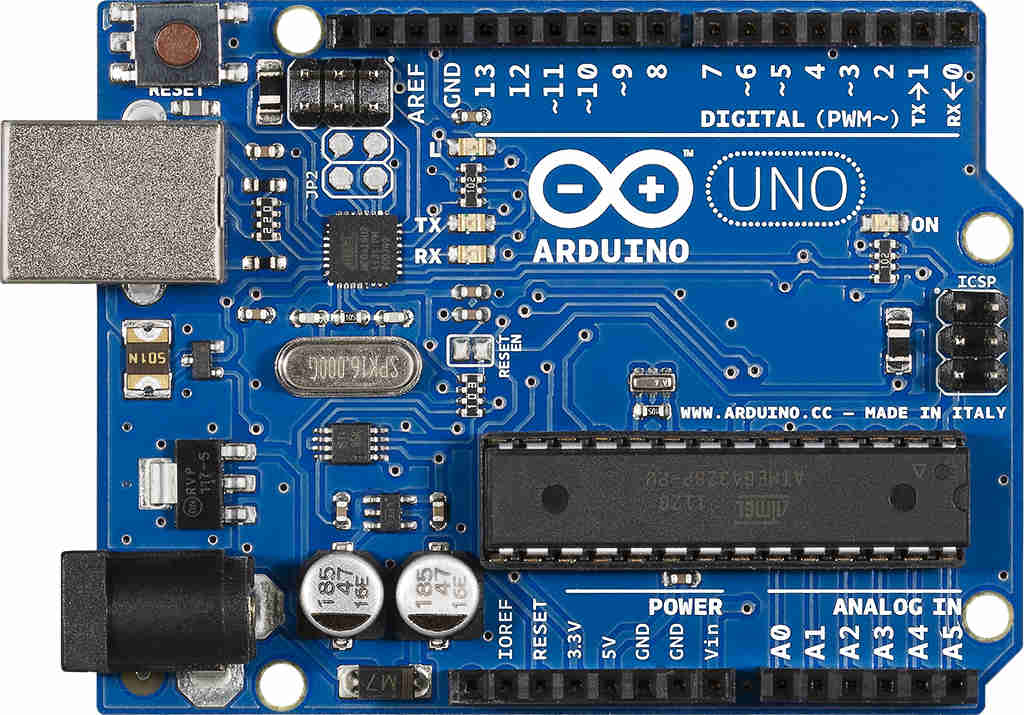
\includegraphics[height=3cm]{ar.jpg}

\section*{ii.RF 433MHz Transmitter/Receiver Module}
These RF modules are very popular among the Arduino tinkerers. The 433MHz transceiver/receiver modules are used on a wide variety of applications that require wireless control.

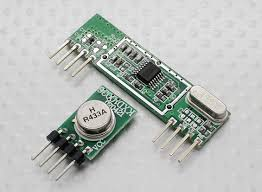
\includegraphics[height=5cm]{download.jpg}
\pagebreak
\section*{iii.MPU6050 Gyro Sensor}
MPU6050 sensor has many functions over the single chip. It consists a MEMS accelerometer, a MEMS gyro, and temperature sensor.This MPU6050 module is a compact chip having both accelerometer and gyro. This is a very useful device for many applications like drones, robots, motion sensors.

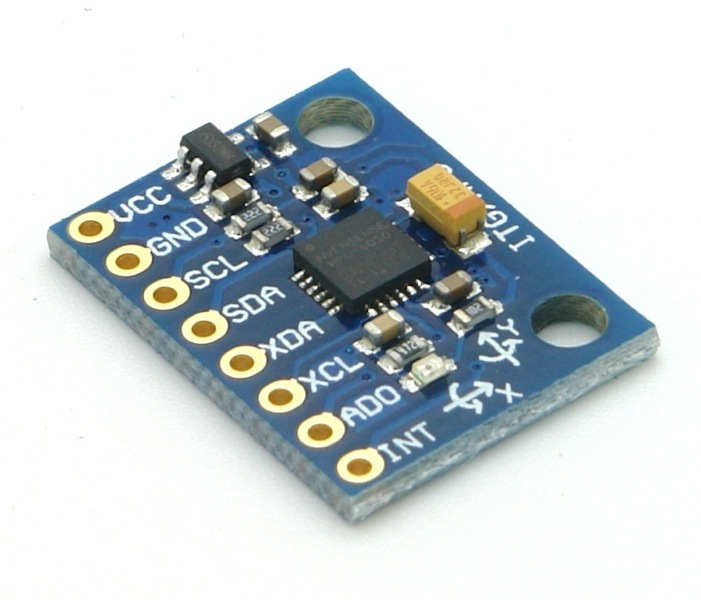
\includegraphics[height=5cm]{MP.jpg}

\section*{iV.L298N Driver}
L298N Driver. The L298N is a dual H-Bridge motor driver which allows speed and direction control of two DC motors at the same time. The module has two screw terminal blocks for the motor A and B, and another screw terminal block for the Ground pin, the VCC for motor and a 5V pin which can either be an input or output.

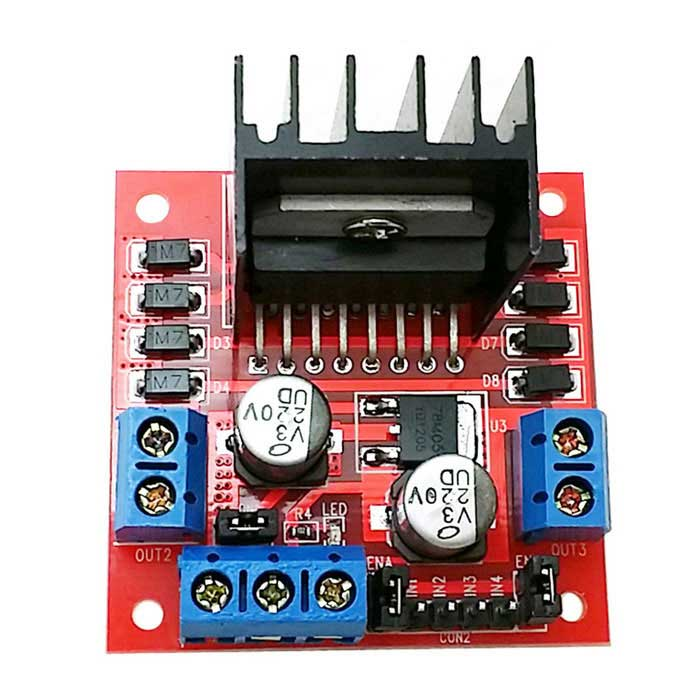
\includegraphics[height=5cm]{L.jpg}
\pagebreak
\section*{V.DC Motor and Wheel}
DC Gear Motor and Wheel. Our DC gear motor and wheel set for making robots! These motors are light weight, high torque and low RPM. They can climb hills and have excellent traction, plus you can mount the wheel on either side of the motor with its double-sided output shaft.

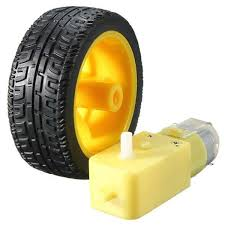
\includegraphics[height=4cm]{Ca.jpg}

\section*{Vi.Mini Breadboard}
Anatomy of a Mini Breadboard. ... These tie points take the form of holes within the breadboard, into which wires and components can be pushed. They're useful for basic prototyping, but breadboards don't accommodate anything with two closely spaced rows of pins, such as the header on the Raspberry Pi.

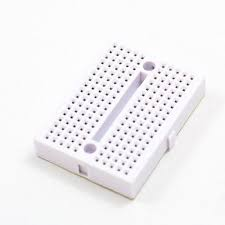
\includegraphics[height=4cm]{B.jpg}

\pagebreak
\section*{Vii.Jumper Wires}
A jump wire (also known as jumper wire, or jumper) is an electrical wire, or group of them in a cable, with a connector or pin at each end (or sometimes without them – simply "tinned"), which is normally used to interconnect the components of a breadboard or other prototype or test circuit, internally or with other equipment or components, without soldering

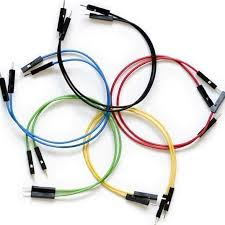
\includegraphics[height=4cm]{J.jpg}

\section*{Viii.Car Chassis Kit}
Size: 22 x 12cm (L x W).
Wheel Size: 6.5cm (Dia.) x 2.7cm (H)
Mechanical structure is simple, it is easy to install.
Can be used for distance measurement, velocity
Can use with other devices to realize function of tracing, obstacle avoidance, distance testing, speed testing, wireless remote control.
Gear Motor reduction radio: 1:48.

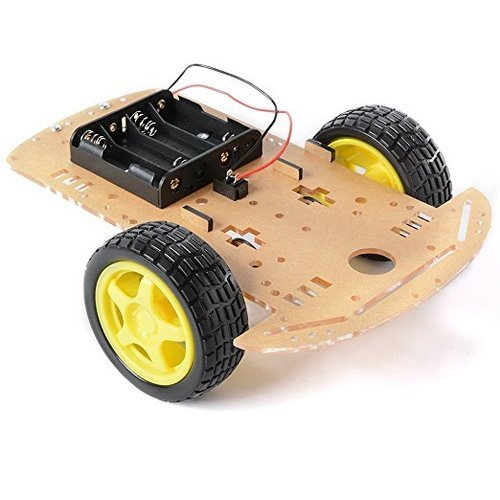
\includegraphics[height=5cm]{C.jpg}
\pagebreak
\section*{ix.18650 Battery Holder}
18650 Battery Holder - Wire - 2 Cell. This 18650 battery case holds two (2) 18650 lithium-ion batteries connected in series, providing approximately 7V output (~3.7V x 2). The holder includes output leads approximately 6" long for soldering or connecting to your circuit.

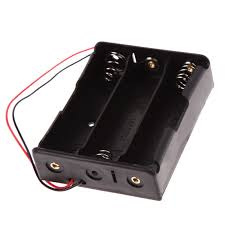
\includegraphics[height=2cm]{BE.jpg}

\section*{x.18650 3.7v Li-Ion Battery}
EBL 18650 3.7V Li-ion Rechargeable Batteries 4 Counts with iQuick 18650 16340.Skywolfeye 18650 Rechargeable Batteries.

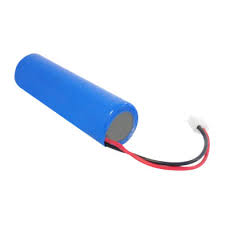
\includegraphics[height=3cm]{BEE.jpg}

\section*{xi.Roller Bovine Wheel}
Overview of Wheels Used in Robotics. The wheel is the most common moving element among other possibilities including legs, flying, swimming and rolling. A wheel provides at least speed, accuracy and stability for a robot, three characteristics very important in designing and build robots.

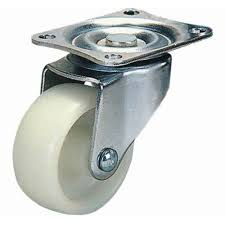
\includegraphics[height=3cm]{1CA.jpg}

\pagebreak
\section{SYSTEM ARCHITECTURE}
Transmitter

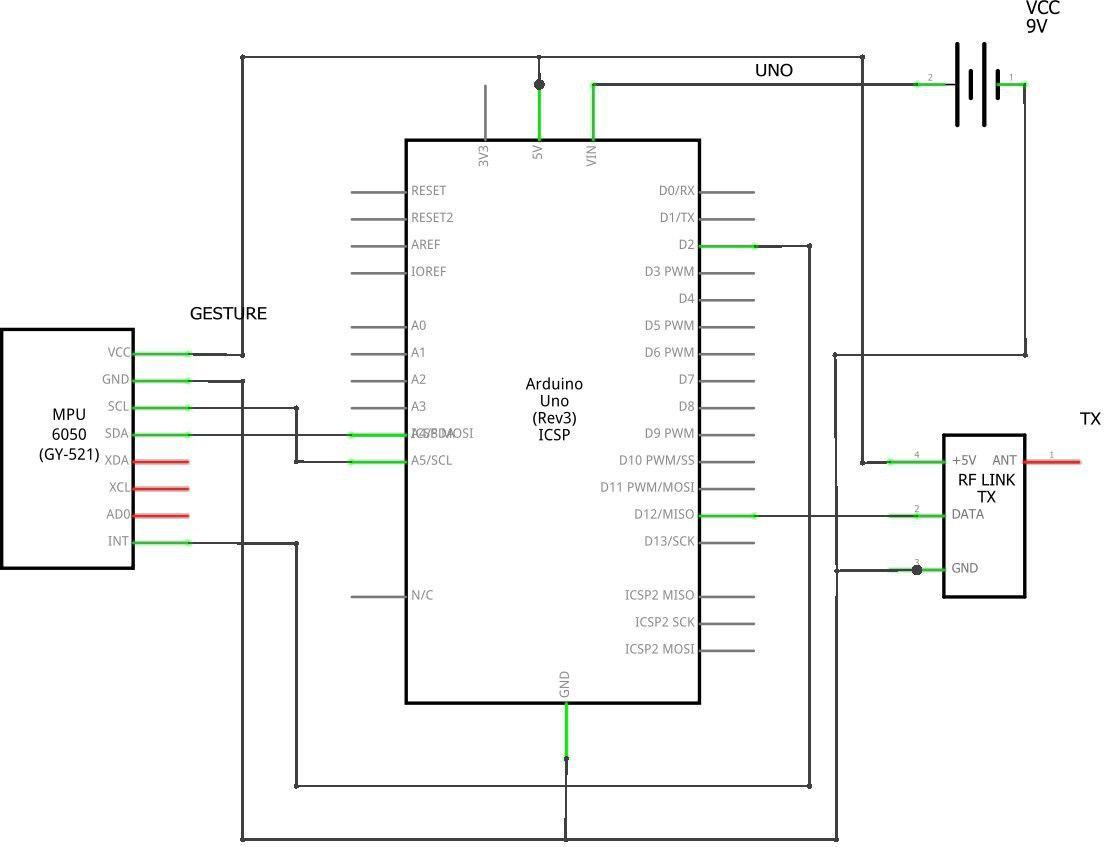
\includegraphics[height=5in]{ta.jpg}
\pagebreak

Receiver

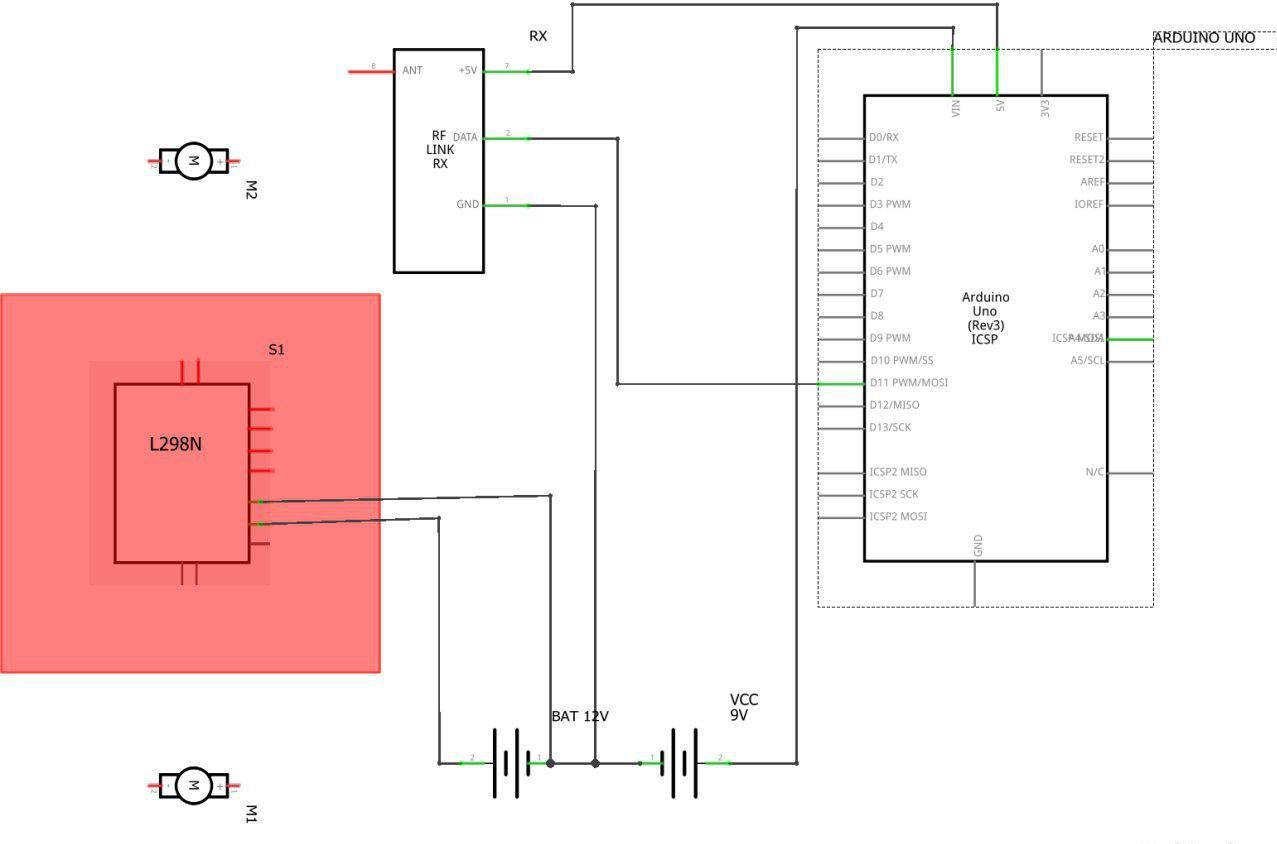
\includegraphics[height=4in]{re.jpg}

\pagebreak

\section{WORKING PROCESS}
In this project, a robot that is controlled by the gestures made by the hand, is designed. The working of the robot is explained here.\newline

As mentioned earlier, the gesture controlled robot is a wireless operated robot and has two parts: Transmitter and Receiver. When the robot is powered on, the transmitter part, which consists of Arduino, MPU6050, Encoder and RF Transmitter, will continuously monitor the MPU6050 sensor.\newline

This data is captured by the Arduino, which then transmits a corresponding data to the Encoder, based on the orientation of the MPU6050 Sensor. The parallel data received by the encoder is converted into serial data and this serial data is transmitted by the RF Transmitter.\newline

At the receiver section, the RF Receiver receives the serial data and transmits it to the Decoder IC. The Decoder will convert the serial data to parallel data and this parallel data is given to the motor driver IC. Based on the data, the movement of the motors, and hence the movement of the robot is defined
\pagebreak


\section{RESULT}
We achieved our object without any hurdles the control of a robot using gesture. The robot is showing proper response whenever we move our hand .Different hand gesture to make the robot move in specific direction are as follow:

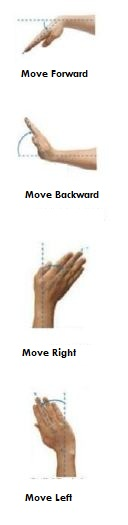
\includegraphics[scale=1.2]{move1.png}

\pagebreak

\section{FUTURE SCOPE}
Future work will build upon the improvement of the correctly recognized the gestures. One approach might be the
implementation of a gyroscope into the system, in order to separate the acceleration due to gravity from the inertial
acceleration and second approach can be that we can install a GPS in the system to track the position of robot. The use
of more accelerometers attached to the arms is another possibility.


\section{CONCLUSION}
Hand Gesture Control becomes an example of companionship between man and machine in the race of man vs.
Machine further enhancing the technology to the next level from Speech recognitions and wired connections to wireless
hand gesture control technology. There is a rapid growth on application development considering gesture recognition
system. So in this paper, we propose a model of a robot based on “Human Gesture Recognition” utilizing hand gestures to communicate with the robot. The 3- axis accelerometer selected to be the input device of this system captures the
human gestures. When compared with the other input devices accelerometer is easier to work and offers the possibility to
control a robot by wireless means. The low price and short set-up time are other advantages of the system but an
important limitation to consider is the reliability of the system. Physical hardship to the user is avoided through the
use of accelerometer as with the twist of the hand, the user gets the ability and freedom to turn the robot into the desired
direction.



\newpage
\bibliographystyle{plain}
\bibliography{biblist}

\end{document}
